%%%%%%%%%%%%%%%%%%%%%%%%%%%%%%%%%%%%%%%%%%%%%%%%%%%%%%%%%%%%%%%%%%%%%%%%%%%%%%

\documentclass{l3deliverable}

%%%%%%%%%%%%%%%%%%%%%%%%%%%%%%%%%%%%%%%%%%%%%%%%%%%%%%%%%%%%%%%%%%%%%%%%%%%%%%

\usepackage{graphicx}%

%%%%%%%%%%%%%%%%%%%%%%%%%%%%%%%%%%%%%%%%%%%%%%%%%%%%%%%%%%%%%%%%%%%%%%%%%%%%%%
%% See D1 for an example of how to integrate sub version revision
%% numbers into a LaTeX document.
%

\version{3}


\usepackage{url}%

%%%%%%%%%%%%%%%%%%%%%%%%%%%%%%%%%%%%%%%%%%%%%%%%%%%%%%%%%%%%%%%%%%%%%%%%%%%%%%
%% Check these macro values for appropriateness for your own document.

\title{Maintenance Report}

\author{Hector Grebbell \\
        Dan Tomosoiu \\
        Peeranat Fupongsiripan
        }

\date{28 February 2013}

\deliverableID{D8}
\project{PSD3 Group Exercise 2}
\team{L}

%%%%%%%%%%%%%%%%%%%%%%%%%%%%%%%%%%%%%%%%%%%%%%%%%%%%%%%%%%%%%%%%%%%%%%%%%%%%%%

\begin{document}

%%%%%%%%%%%%%%%%%%%%%%%%%%%%%%%%%%%%%%%%%%%%%%%%%%%%%%%%%%%%%%%%%%%%%%%%%%%%%%

\maketitle

\tableofcontents

\newpage

%%%%%%%%%%%%%%%%%%%%%%%%%%%%%%%%%%%%%%%%%%%%%%%%%%%%%%%%%%%%%%%%%%%%%%%%%%%%%%
%% Standard section for all documents

\section{Purpose and Description of Document}
This report documents maintenance improvements to our Intern Management System implementation. \\
Due to updating of system requirements by the client it became necessary to make several adjustments to the implementation.\\

\subsection{Changes to system requirements}

\begin{itemize}
\item A student should be able to accept multiple approved internships, provided their dates do not overlap.
\item Students must have sufficient approved internships to cover a total of at least 12 weeks.
\item Addition of the WITHDRAWN status for each role.
\item The same academic visitor must visit all internships assigned to a single student.
\end{itemize}

\section{Changes}

\subsection{Role Implementation}

\subsubsection{Role Status}
Approval status changed from a boolean value to an enum (PENDING, APPROVED, WITHDRAWN) due to changes to system requirements.

\subsubsection{Role Status}
Added grade variable (To allow removal of Visit class) for assignment by visitor due to changes to system requirements.

\subsection{Placement Implementation}

\subsubsection{Placement Role}
Role changed from singular to array, allowing several roles to be assigned to the same students placement. Change necessary due to changes to system requirements.

\subsubsection{Addition of Approval}
Boolean value added to indicate whether placement has been approved by the coordinator. Change necessary due to changes to system requirements.

\subsubsection{Addition of Internship Duration Constraint}
To be approved a students combined placement roles must sum to at least 12 weeks in duration. Change necessary due to changes to system requirements.

\subsubsection{Addition of updateRoleStatus Method}
Method added to allow employers to approve a student for a role. Change necessary due to changes to system requirements.

\subsection{Visitor Implementation}

\subsubsection{Assignment to Students}
Addition of array of students (to allow removal of Visit class) which the visitor is assigned to. Change necessary due to changes to system requirements.

\subsubsection{Addition of assignPlacementGrade Method}
Method added to allow a visitor to assign a grade to one of the students he is visiting. Change necessary due to changes to system requirements.

\subsection{Changes to Class Diagrams}
Due to changes to the specification the Placement Store API changed somewhat. Hence the class diagram was updated as below.

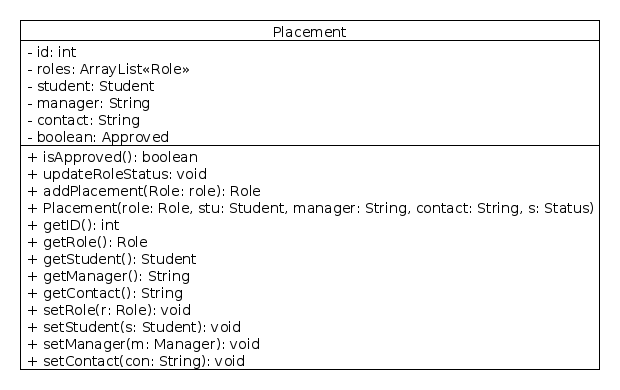
\includegraphics[scale = 1]{ClassDiagram_PlacementStore.png}\\


\section{Changes to the API and potential future changes}

\subsection{API Changes}
Because of the changes made, some API calls needed to be changed:
\begin{itemize}
\item IsApproved() method of the Role interface changed to getStatus(), since there are three possible status a role might have. The returning type is Status instead of the initial boolean type. To respect backwards-compatibility, the isApproved() method has been left as a method, returning true if the Status is APPROVED or false if it is WITHDRAWN or PENDING.
\item Placement constructor was updated to take the additional Status parameter.
\item Grade attribute was added so the Role had to be updated as well as a consequence.
\item Visitor class was updated to have each visitor hold a list of the students to which they have been allocated for visits.
\end{itemize}

\subsection{Acceptance Test}
Because of the changes made, the following changes to the acceptance tests should be done:
\begin{itemize}
\item Additional tests need to be written for when a student withdraws his application for a role.
\item Tests should be added for a visitor to set a grade for a visit to a student's role. 
\item Test should be added for the case where a student has multiple roles, and also check coordinator approval only being possible if their total duration is at least 12 weeks.
\item Multiple roles added to the same placement need to be checked for overlapping.
\item Since employers can also approve students for a role, further tests should be written for this.
\end{itemize}


\end{document}

%%%%%%%%%%%%%%%%%%%%%%%%%%%%%%%%%%%%%%%%%%%%%%%%%%%%%%%%%%%%%%%%%%%%%%%%%%%%%%
